\subsection{One-Dimensional Model}

\subsubsection{Diffusion With Consumption}

\textbf{Different Bacterial Concentrations}

\begin{figure}[H]
    \centering
    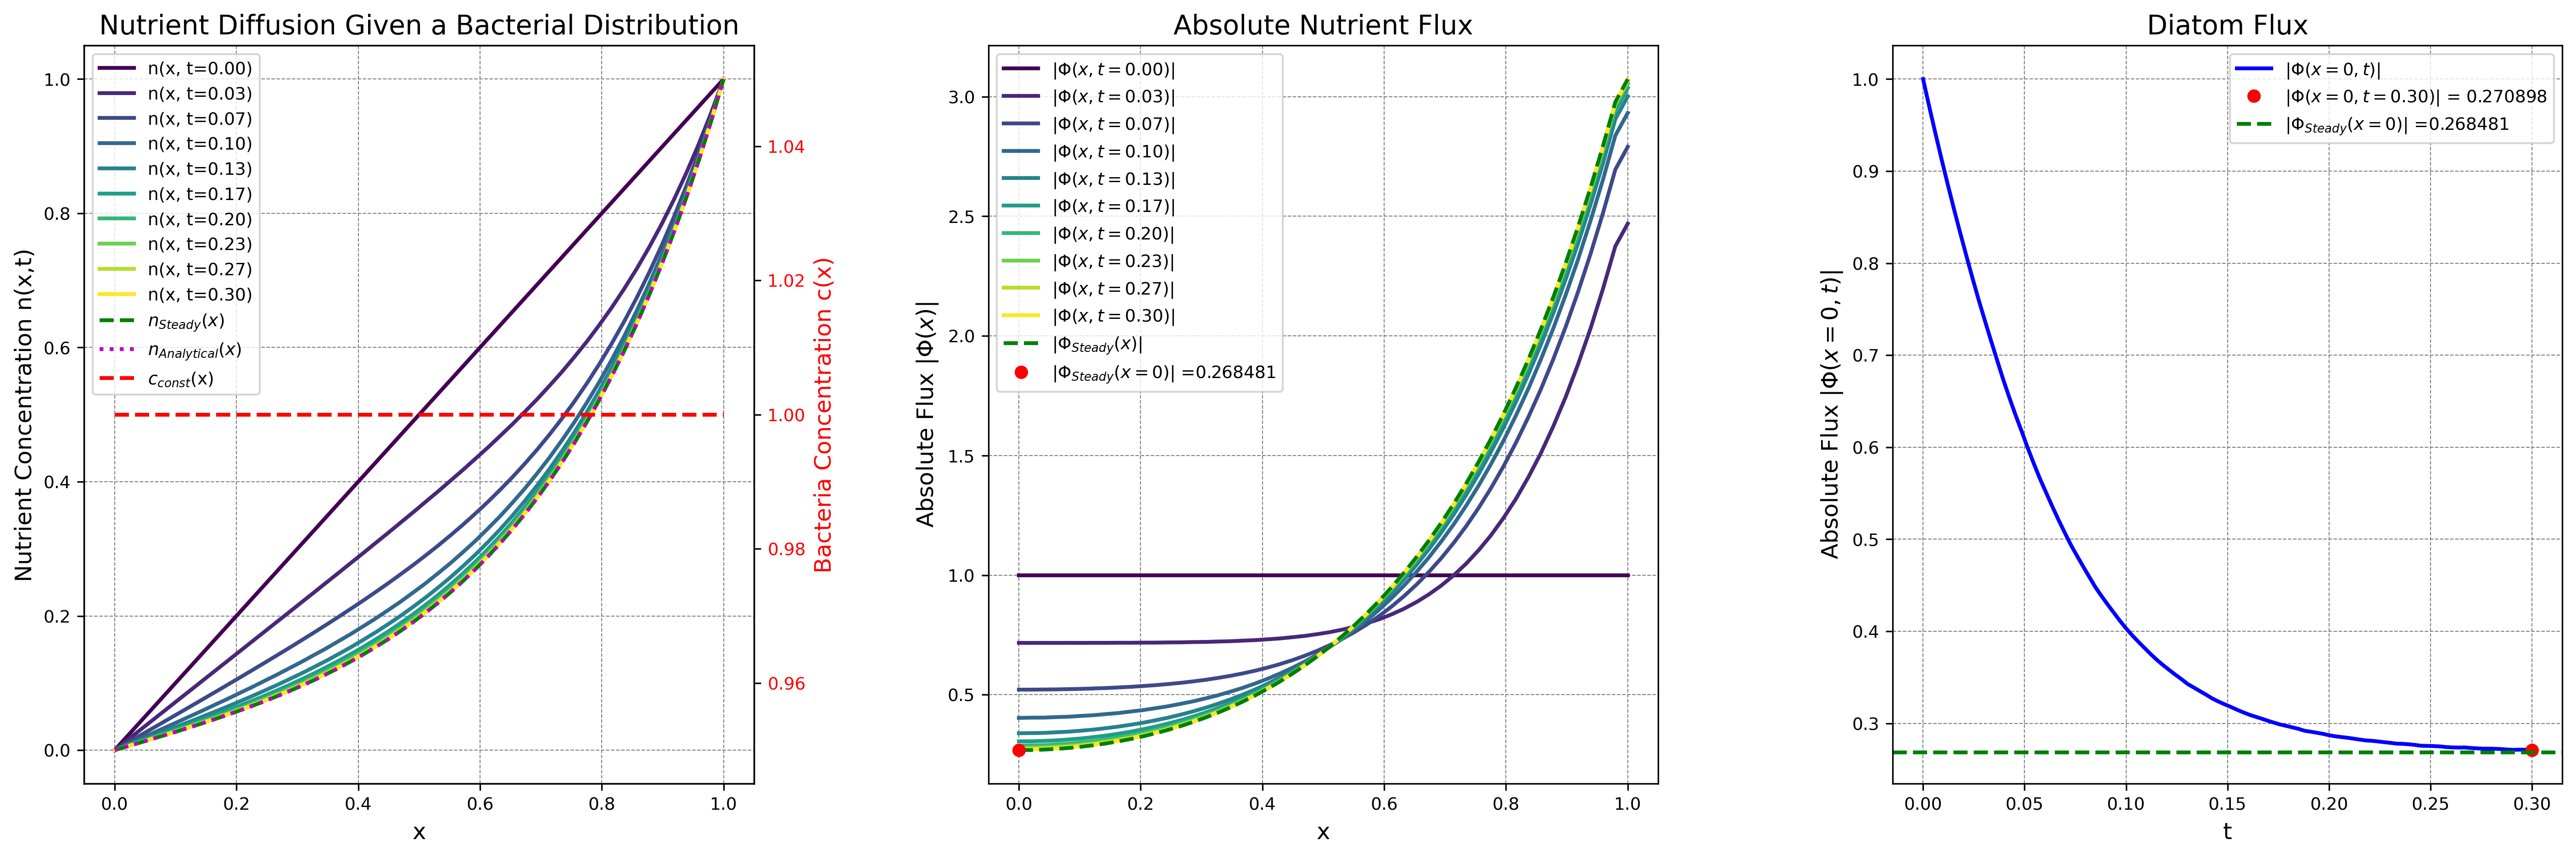
\includegraphics[width=0.8\textwidth]{Figures/c_const(x)_Analyt.png}
    \caption{Constant Bacterial Concentration Profile, with Analytical Solution.}
    \label{fig:c_const}
\end{figure}

\begin{figure}[H]
    \centering
    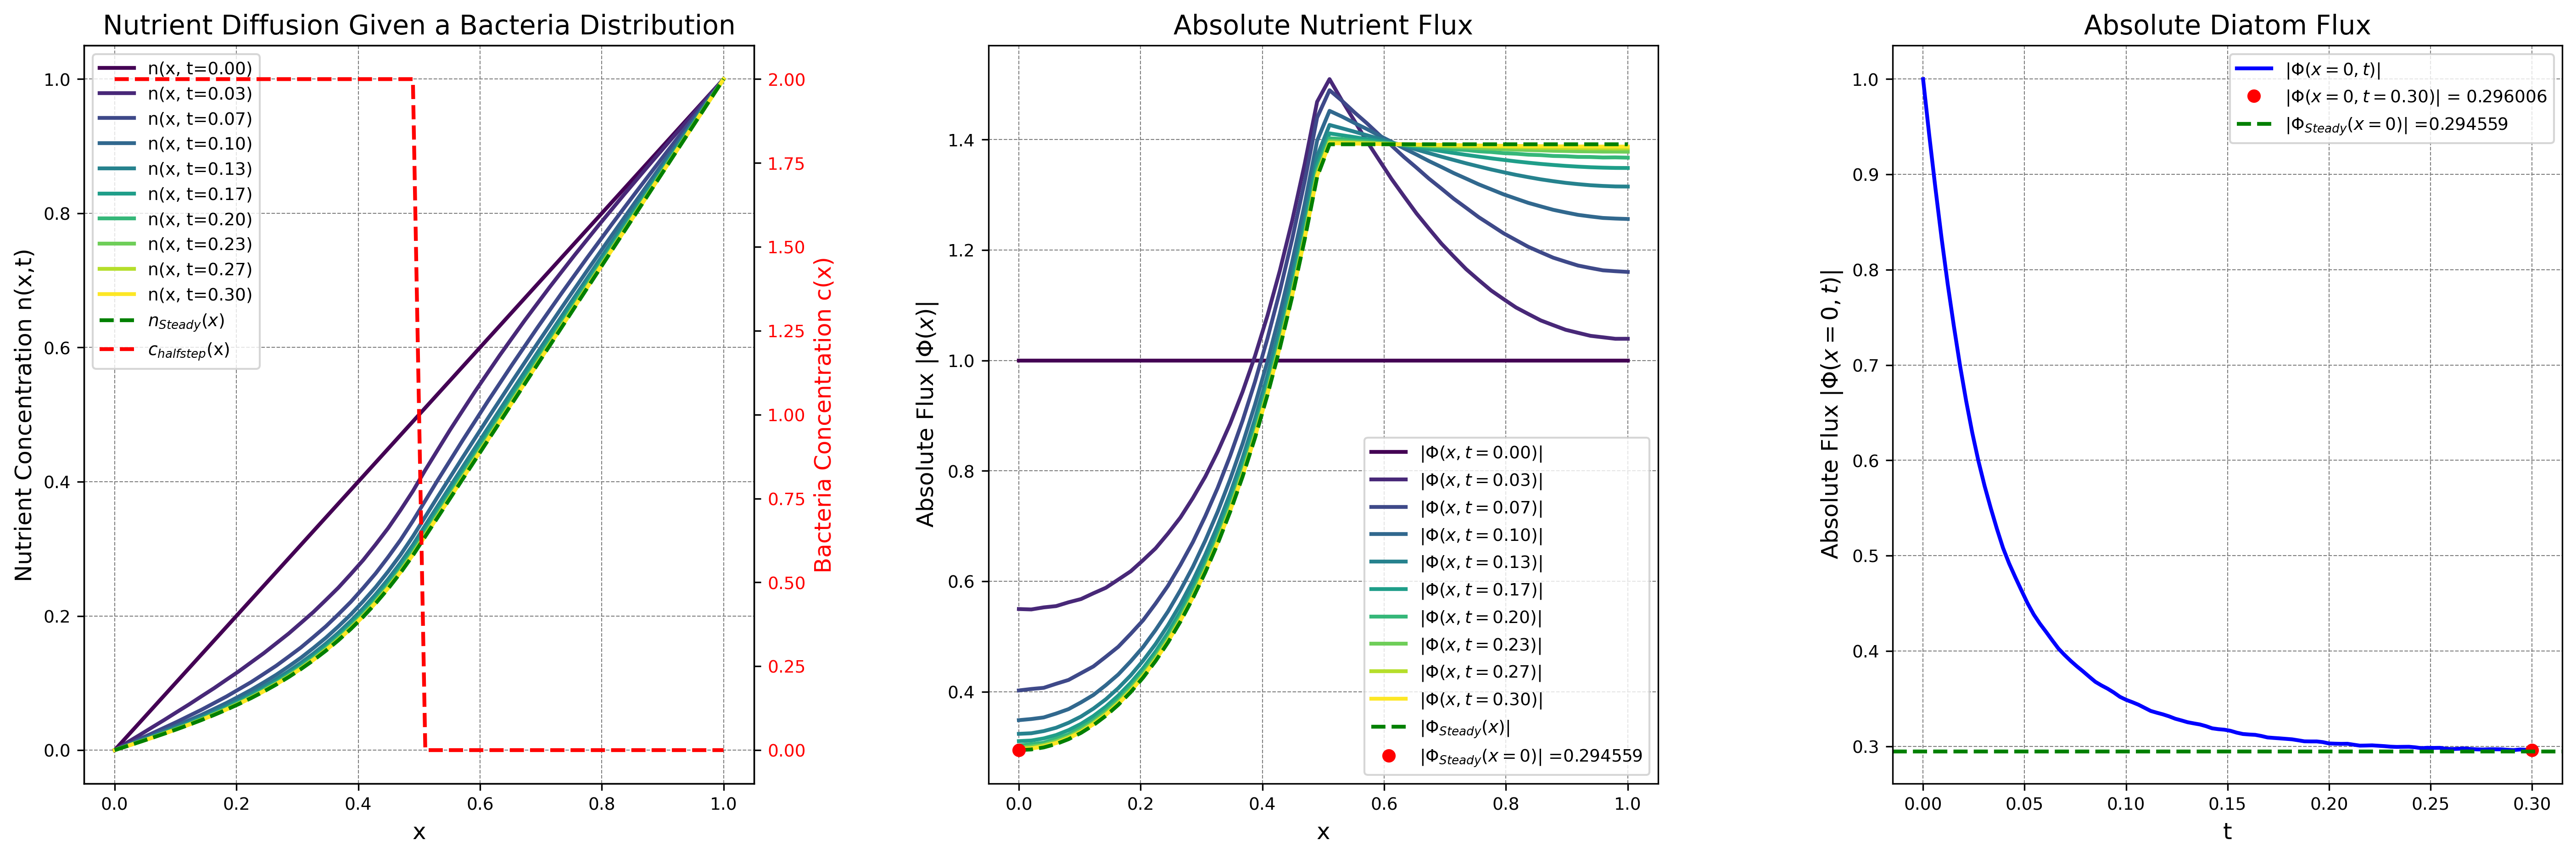
\includegraphics[width=0.8\textwidth]{Figures/c_halfstep(x).png}
    \caption{Half-Step Bacterial Concentration Profile.}
    \label{fig:c_halfstep}
\end{figure}

\begin{figure}[H]
    \centering
    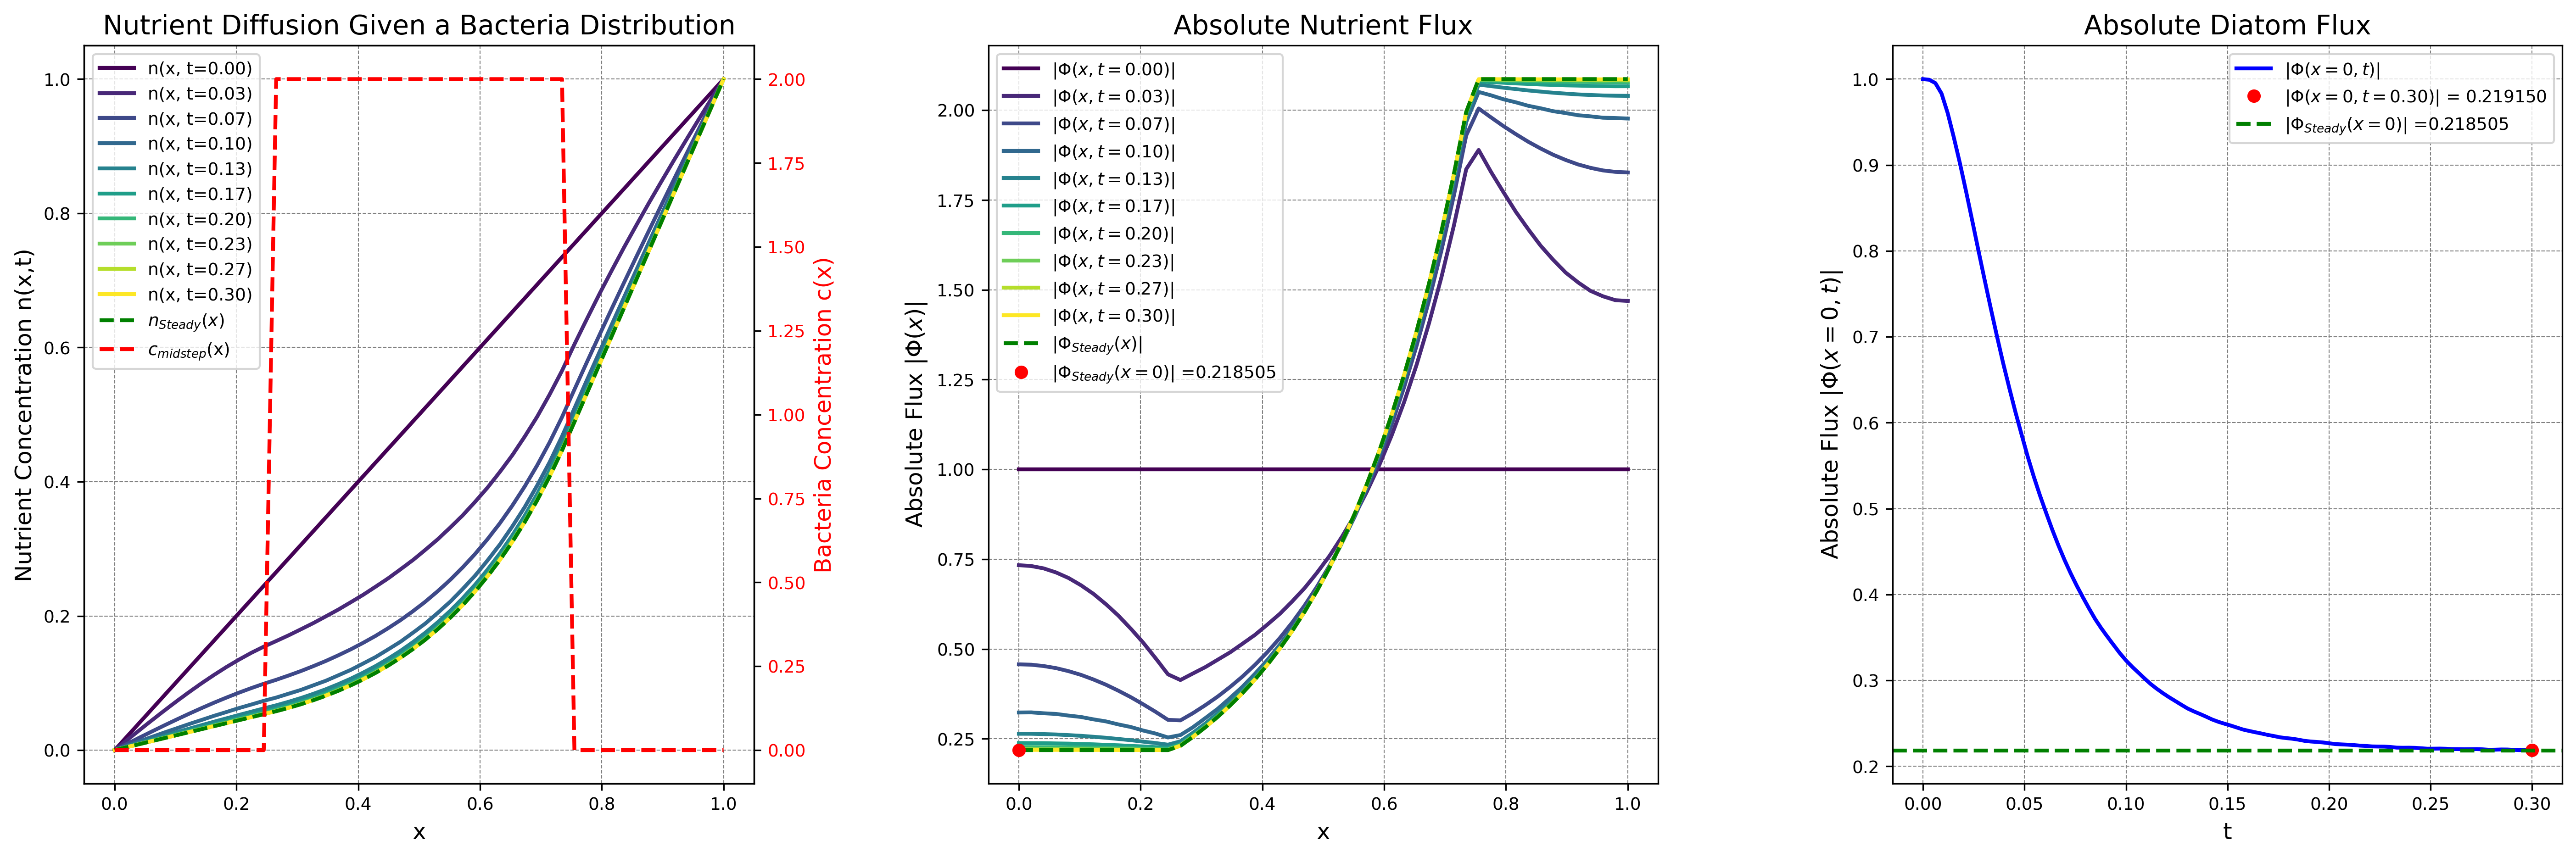
\includegraphics[width=0.8\textwidth]{Figures/c_midstep(x).png}
    \caption{Mid-Step Bacterial Concentration Profile.}
    \label{fig:c_midstep}
\end{figure}

\textbf{ \color{red} ¿Different Diffusion Coefficients?}

\begin{figure}[H]
    \centering
    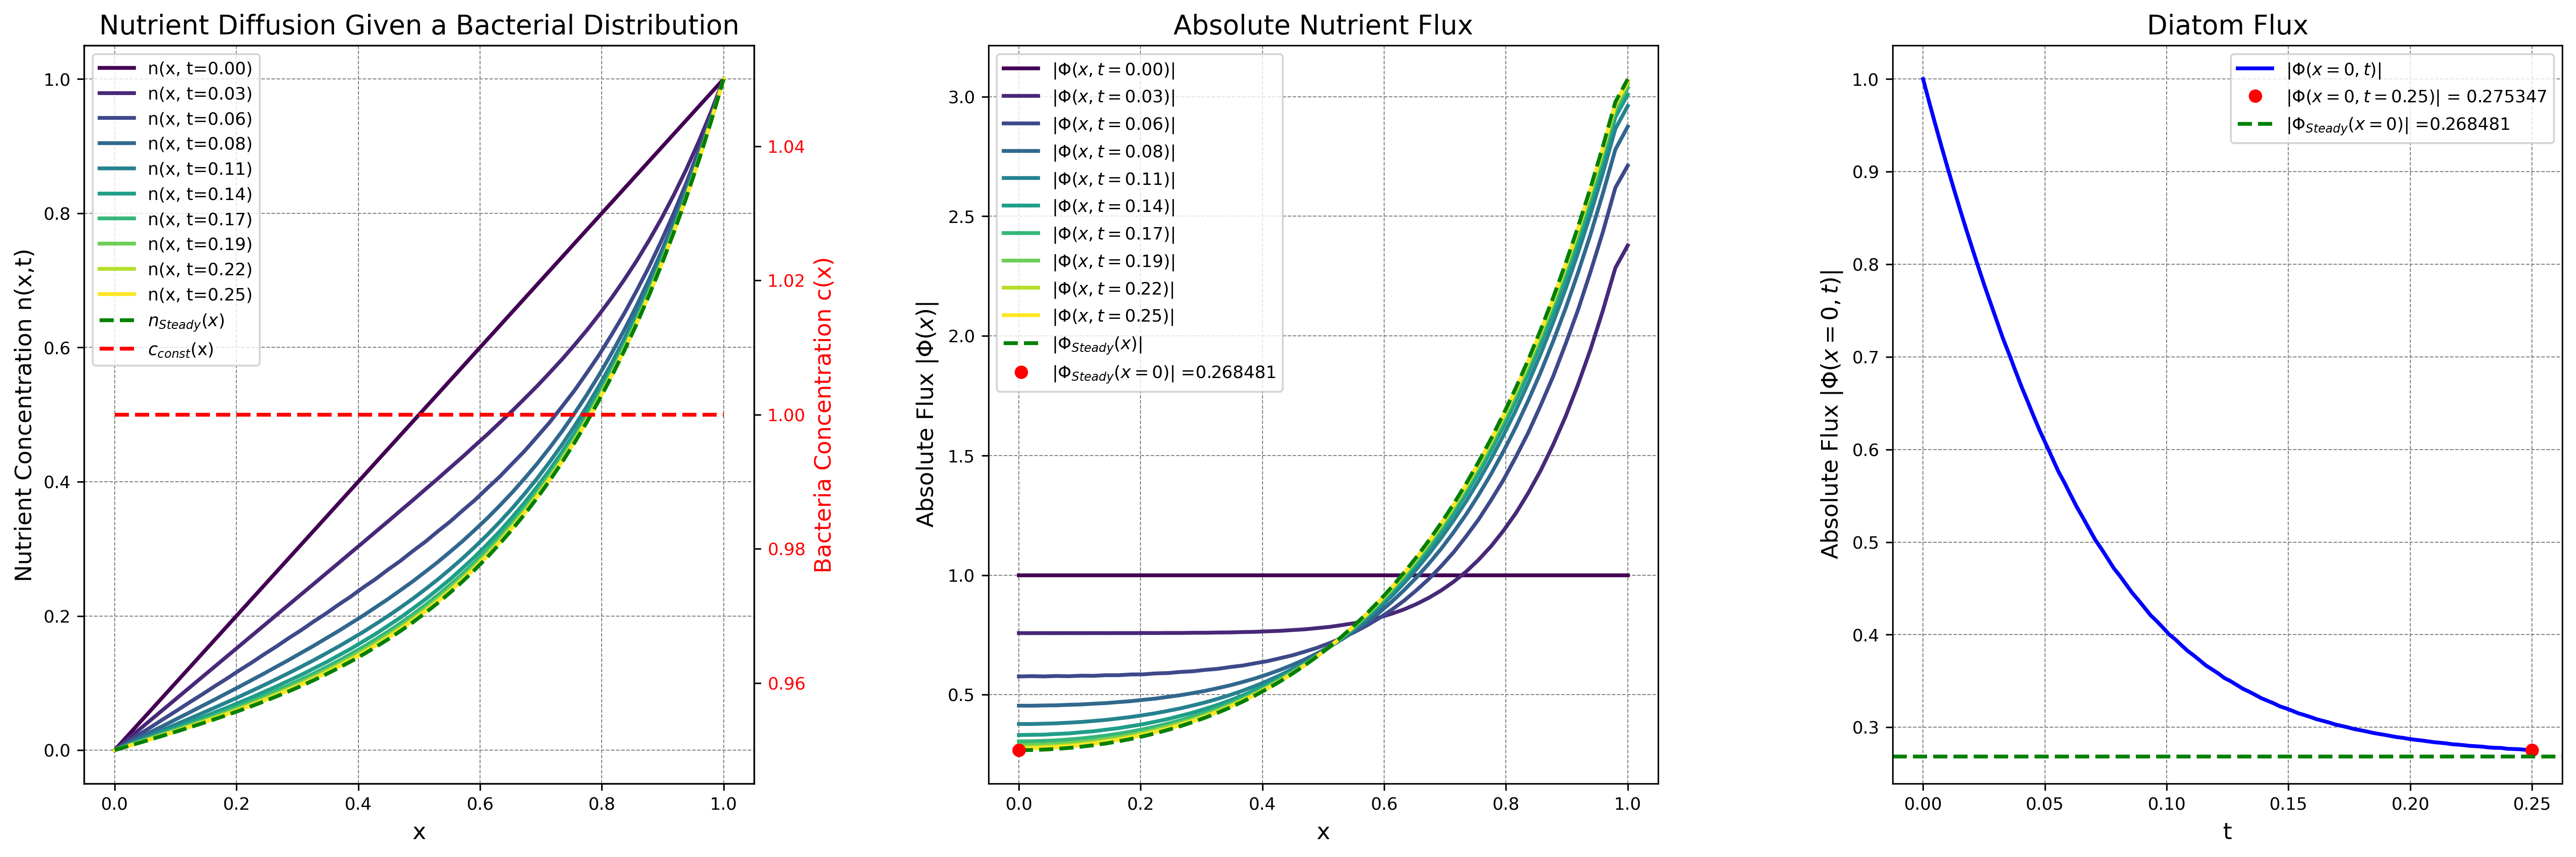
\includegraphics[width=0.8\textwidth]{Figures/Diff_Dom.png}
    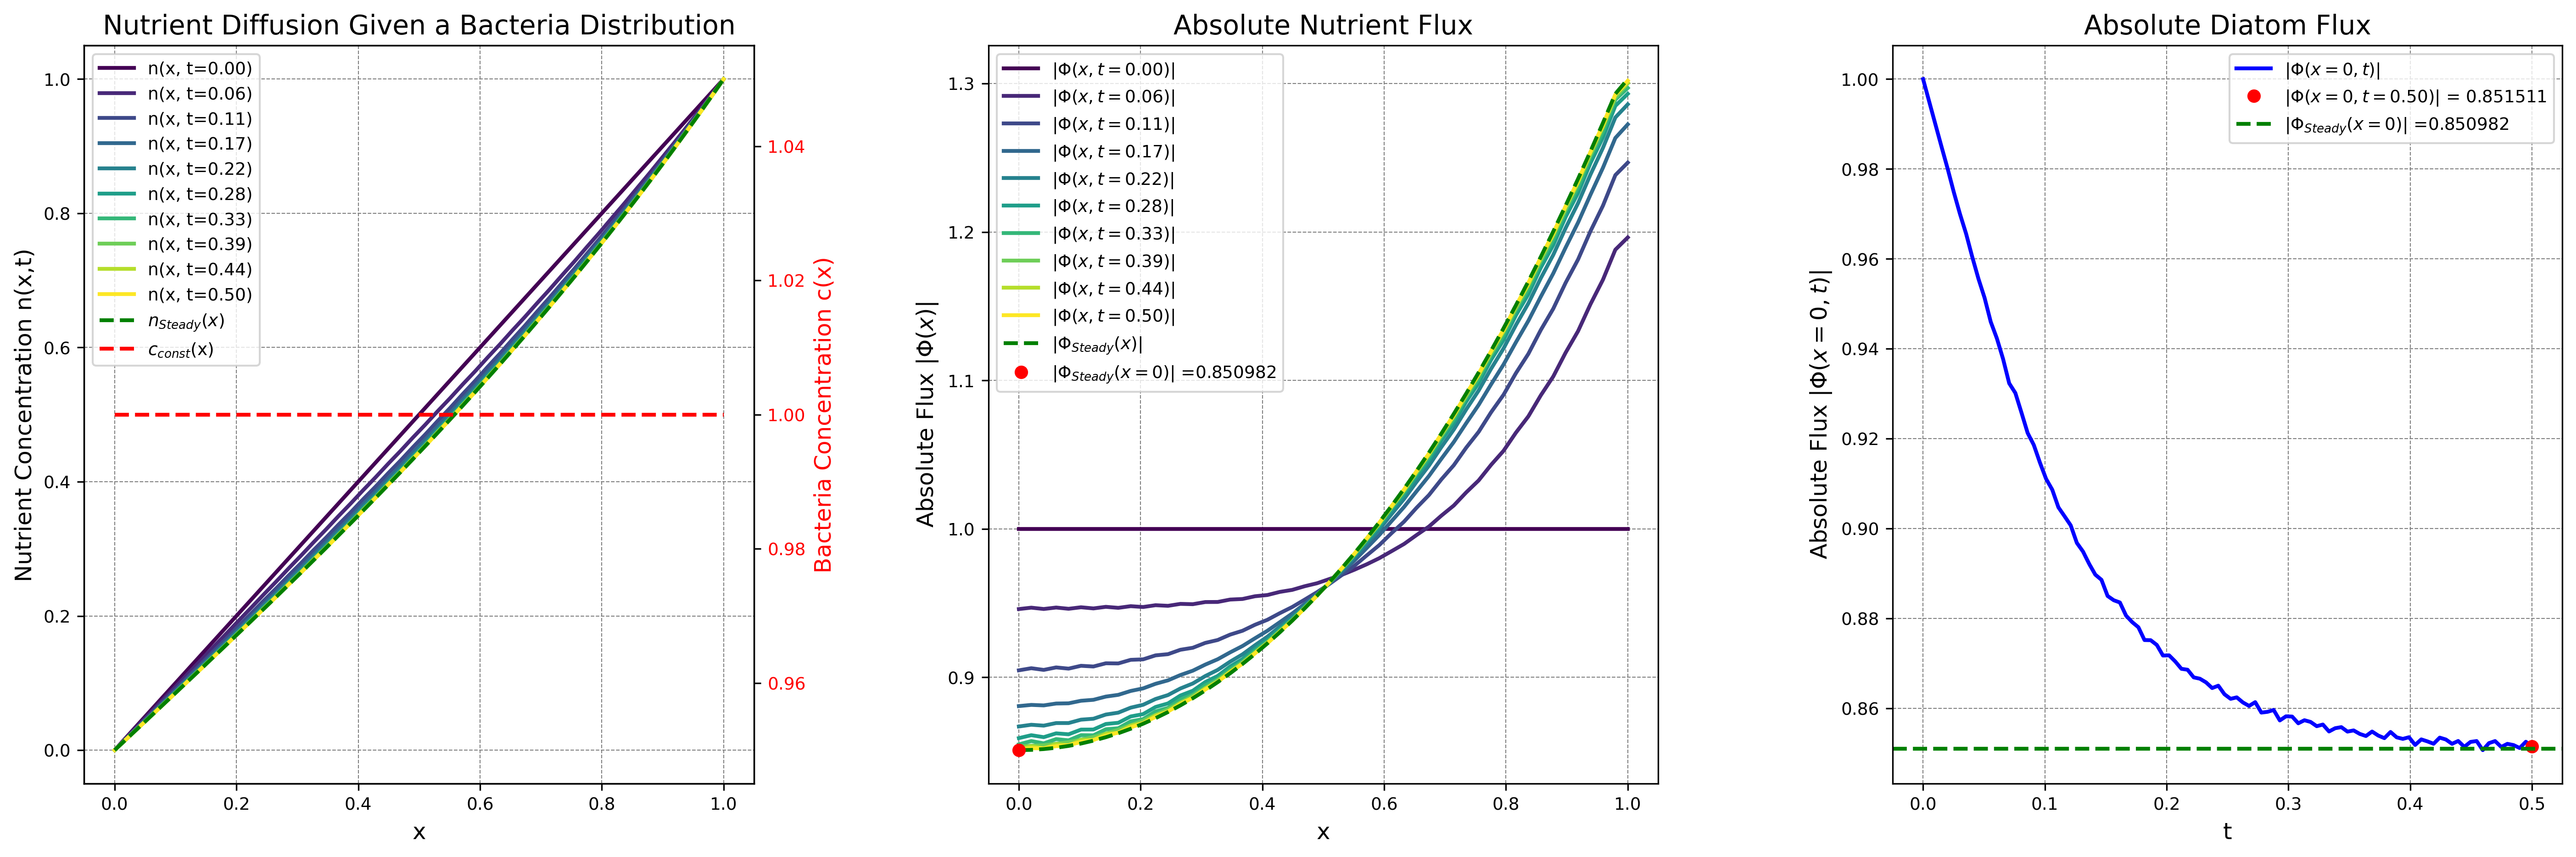
\includegraphics[width=0.8\textwidth]{Figures/Diff~Consump.png}
    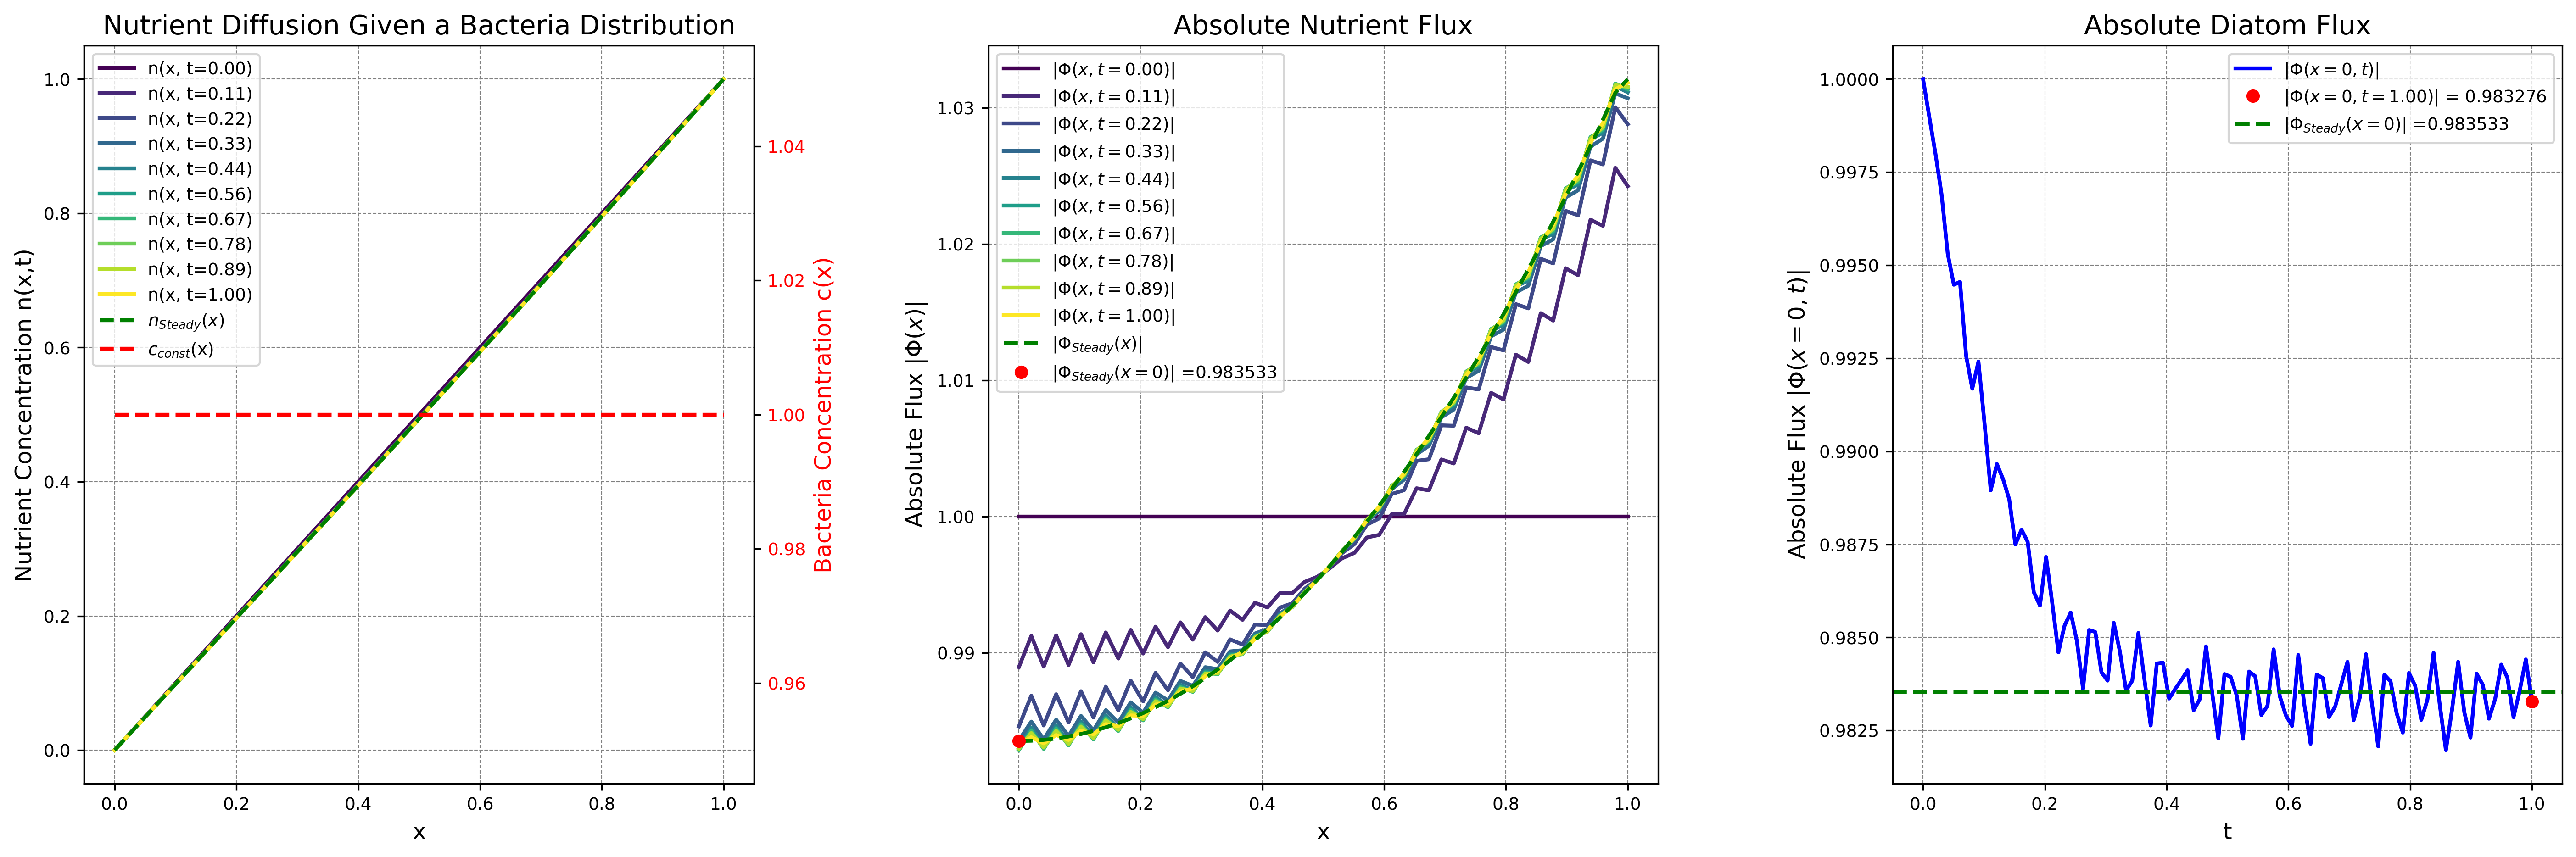
\includegraphics[width=0.8\textwidth]{Figures/Consump_Dom.png}
    \caption{Comparing Different Diffusion-Consumption Ratios.}
    \label{fig:Diff_Consump}
\end{figure}

\textbf{Diatom's FluxMaps, Generalising Results for Step \& Exponential Concentrations}

Concentration profile described by a midstep with varying starting positions ($x_0$) and lenghts ($l$), with the restriction $x_0 + l \leq L$.

\begin{equation}
    c_{\text{midstep}}(x; x_0,l) = 
    \begin{cases} 
    \frac{1}{l} & \text{if } x_0 \leq x \leq x_0 + l, \\
    0 & \text{otherwise}.
    \end{cases}
\end{equation}

\begin{figure}[H]
    \centering
    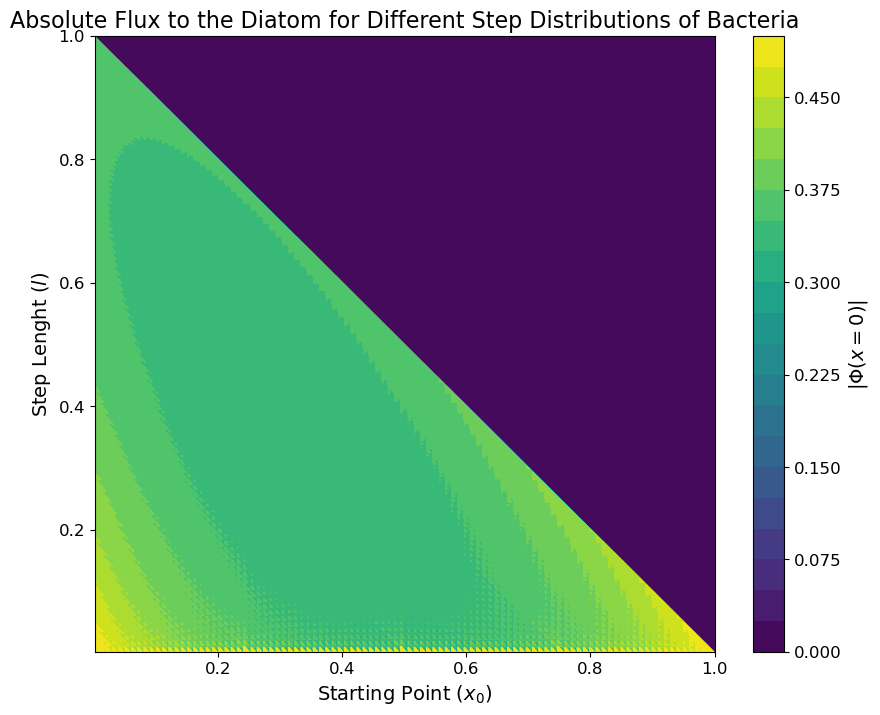
\includegraphics[width=0.6\textwidth]{Figures/FluxMap_midstep.png}
    \caption{Flux Map for Midstep Concentration Profile.}
    \label{fig:FluxMap_midstep}
\end{figure}

Concentration profile described by an exponential with varying slope.

\begin{equation}
    c_{\text{exp}}(x; \delta) =
    \frac{1}{\delta L}
    \frac{\mathrm{e}^{-\frac{x}{\delta L}}}{1 - \mathrm{e}^{-\frac{1}{\delta}}}
\end{equation}

\begin{figure}[H]
    \centering
    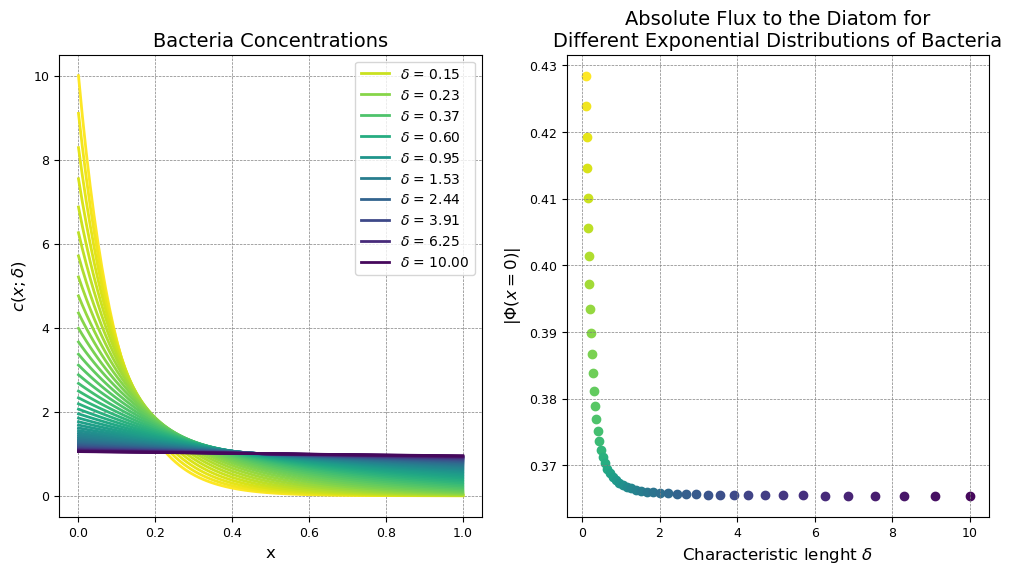
\includegraphics[width=0.6\textwidth]{Figures/FluxMap_exp.png}
    \caption{Flux Map for Exponential Concentration Profile.}
    \label{fig:FluxMap_exp}
\end{figure}

\subsubsection{Absorption of Brownian Particles}

\subsection{Tree-Dimensional Model}

\subsubsection{Numerical Solution}

\subsubsection{Analytical Solution}